\documentclass[10pt]{beamer}
\usetheme{Warsaw}
\usepackage[utf8]{inputenc}
\usepackage[english]{babel}
\usepackage{amsmath}
\usepackage{amsfonts}
\usepackage{amssymb}
\usepackage{graphicx}
\author{inż. Piotr Zdunek\\
dr inż. Grzegorz Kasprowicz}
\title{Camera design framework for scientific applications}
%\titlegraphic{    
%                    
%                     
\includegraphics[width=1.8cm,keepaspectratio]{pic/logoEiTI.png}\hspace*{1,5cm}~
%                     
\includegraphics[width=1.8cm,keepaspectratio]{pw-logo.jpg} \hspace*{1,5cm}~
%                     
\includegraphics[width=1.8cm,keepaspectratio]{pic/logo_ise.png} 
%                     
%                     }
%\setbeamercovered{transparent} 
%\setbeamertemplate{navigation symbols}{} 
\logo{               
\includegraphics[width=1cm,keepaspectratio]{pic/logoEiTI.png}\hspace*{0,5cm}
    
\includegraphics[width=1cm,keepaspectratio]{pw-logo.jpg} \hspace*{0,5cm}
    
\includegraphics[width=1cm,keepaspectratio]{pic/logo_ise.png} \hspace*{0,5cm}
} 
\institute{Warsaw University of Technology\\
    Faculty of Electronics and Information Technology\\
    Institute of Electronic Systems \\ 
Photonics and Web Engineering Group} 
\date{16.03.2017} 
\subject{Master Thesis} 
%\setbeamercovered{transparent} 
%\setbeamertemplate{navigation symbols}{} 
%\logo{} 
%\institute{} 
%\date{} 
%\subject{} 
\begin{document}

\begin{frame}
    \titlepage
\end{frame}

%\begin{frame}
%\tableofcontents
%\end{frame}
%
%\section{Introduction}
\begin{frame}{Agenda}
    \begin{itemize}
        \item Project genesis 
        \item Requirements
        \item Concept of design
        \item Realisation
        \item Tests
        \item Future work
    \end{itemize}

\end{frame}

%\section{Project genesis}

\begin{frame}{$\pi$ of the sky - camera system}

    \begin{figure}[H]
        \centering
        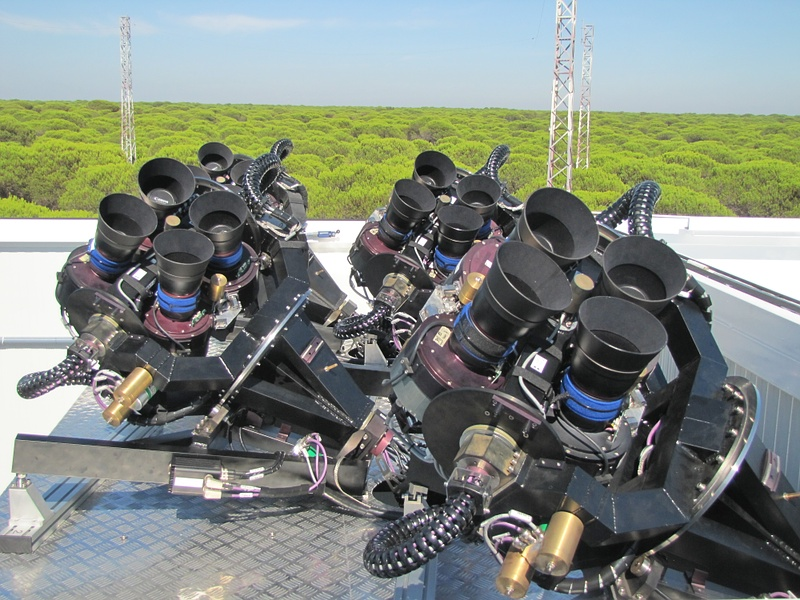
\includegraphics[width=10cm]{pic/camera_pi.jpg}
        \caption{Example of a scientific camera system}
    \end{figure}

\end{frame}


\begin{frame}{Project genesis}

    The goal: provide a faster and easier way to develop camera systems for scientific applications

    General problems when developing camera systems:
    \begin{itemize}
        \item design of electronics for specific MCU
        \item development of software/firmware/digital system design to support a specific sensor
        \item development of data transfer from the sensor to a PC or a storage device
        \item upgrade capability  
    \end{itemize}

\end{frame}
%\section{Requirements}


\begin{frame}{Requirements}

    \begin{enumerate}
        \item \textbf{High data acquisition} - input throughput 600 MB/s (4 MP @ 100 fps, 12 bits per pixel) 
        \item \textbf{Ease of adding a support for a different sensor}
        \item \textbf{High speed communication} 
            \begin{enumerate}
                \item 3 Gbps Serial ATA 
                \item 1 Gbps Ethernet 
            \end{enumerate}
        \item \textbf{Multichannel operation} - Ethernet Precision Time Protocol 
        \item \textbf{Versatile OS}
            \begin{enumerate}
                \item GNU/Linux 
                \item FreeRTOS  
            \end{enumerate}

    \end{enumerate}
\end{frame}
%
%    \begin{frame}{Concept of realisation - Main Processing Unit}
%        Main requirements: 
%        \begin{itemize}
%            \item Camera interface 
%            \item High speed interface for data transmission 
%            \item Ability to run Embedded Linux and an RTOS
%        \end{itemize}
%        \vspace{1cm}
%        The choice of architecture:
%        \begin{itemize}
%            \item use two ICs: an  FPGA and an Application Processing Unit
%            \item use just an FPGA with soft processor done in logic   
%            \item use an SoC with FPGA and APU on one silicon die 
%        \end{itemize}
%    \end{frame}

\begin{frame}{Concept of realisation - Main Processing Unit}
    Xilinx Zynq SoC 
    \begin{itemize}
        \item high processing capability - 2x Cortex A9
        \item high speed connectivity - GTX transceivers - up to 12.5 Gbps per link
        \item versatility - FPGA fabric             
        \item cost optimal - many variants             
        \item future proof - modern solution
    \end{itemize}

    \begin{figure}[H]
        \centering
        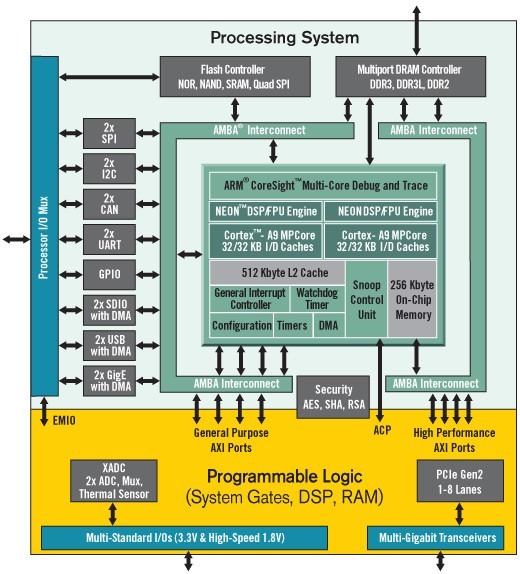
\includegraphics[width=8cm]{pic/zynq.jpg}
        \caption{Zynq Architecture}
    \end{figure}
\end{frame}


    \end{frame}


    \begin{frame}{Concept of realisation}
        Data Interfaces: 
        \begin{itemize}
            \item Serial ATA - using an IP Core from OpenCores.org
            \item 1 Gb Ethernet - using PCS/PMA IP Core (no need to use PHY chip)
        \end{itemize}


        Sensors: 
        \begin{itemize}
            \item CMOSIS CMV4000 2 MPix CMOS Sensor - up 100 fps
            \item Counting detector sensor 
        \end{itemize}

    \end{frame}

    \begin{frame}{Realisation}
        Several subsystems were designed and tested for the project:    

        \begin{itemize}

            \item CMV4000 IP data acquisition for ZC706
            \item Dual SSD Serial ATA data storage
            \item FreeRTOS/AMP on ZC706        
            \item Counting Sensor IP data acquisition
            \item Petalinux desgin 
            \item PCS/PMA 1 GbE  data transfer

        \end{itemize}

    \end{frame}

    \begin{frame}{Realisation}

        \begin{minipage}{.5\textwidth}
            \centering
            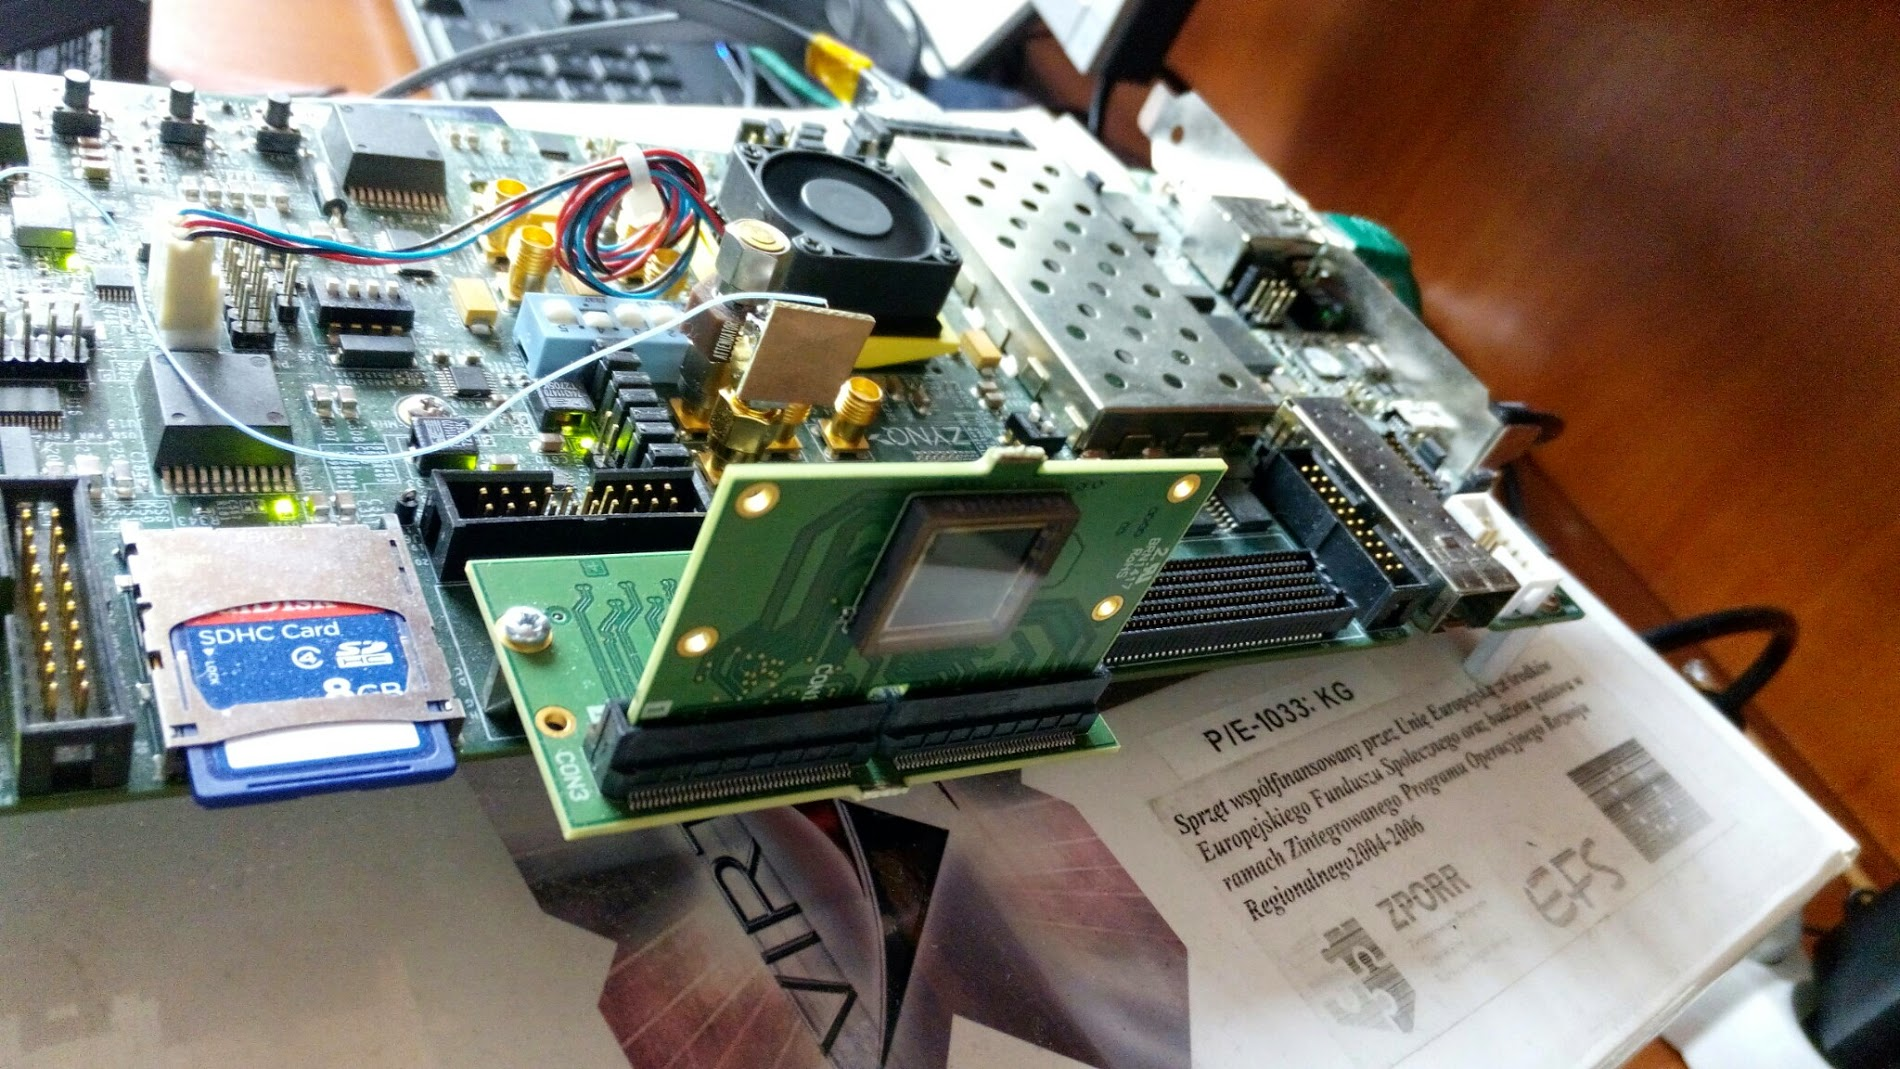
\includegraphics[width=5cm]{pic/zc706_cmv_4000.jpg}\\
            \caption{CMOS sensor system}
        \end{minipage}%
        \begin{minipage}{0.5\textwidth}
            \centering
            \includegraphics[width=5cm]{pic/zc706_counting.JPG}\\
            \caption{Counting sensor system}
        \end{minipage}

    \end{frame}

    \begin{frame}{Realisation}

        \begin{minipage}{.5\textwidth}
            \centering
            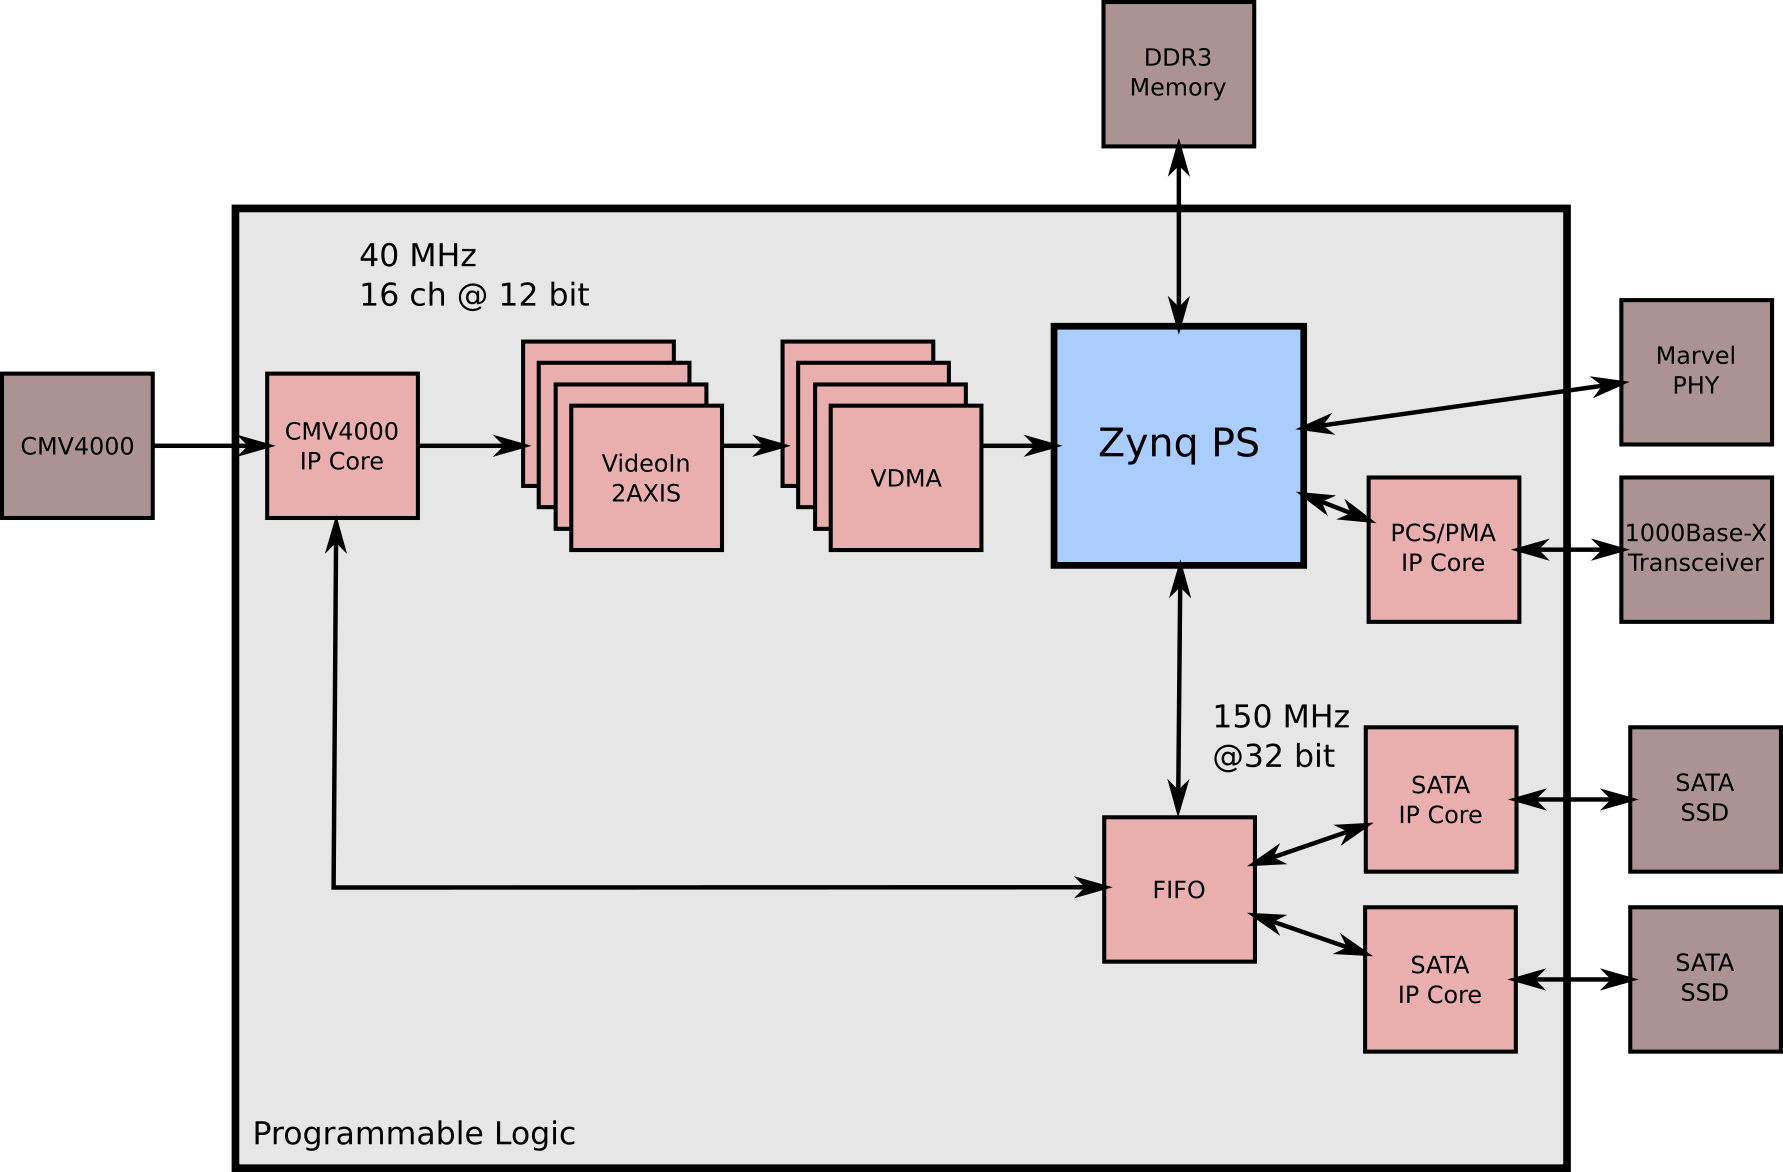
\includegraphics[width=5cm]{pic/cmv4000_arch.png}\\
            \caption{CMOS arch.}
        \end{minipage}%
        \begin{minipage}{0.5\textwidth}
            \centering
            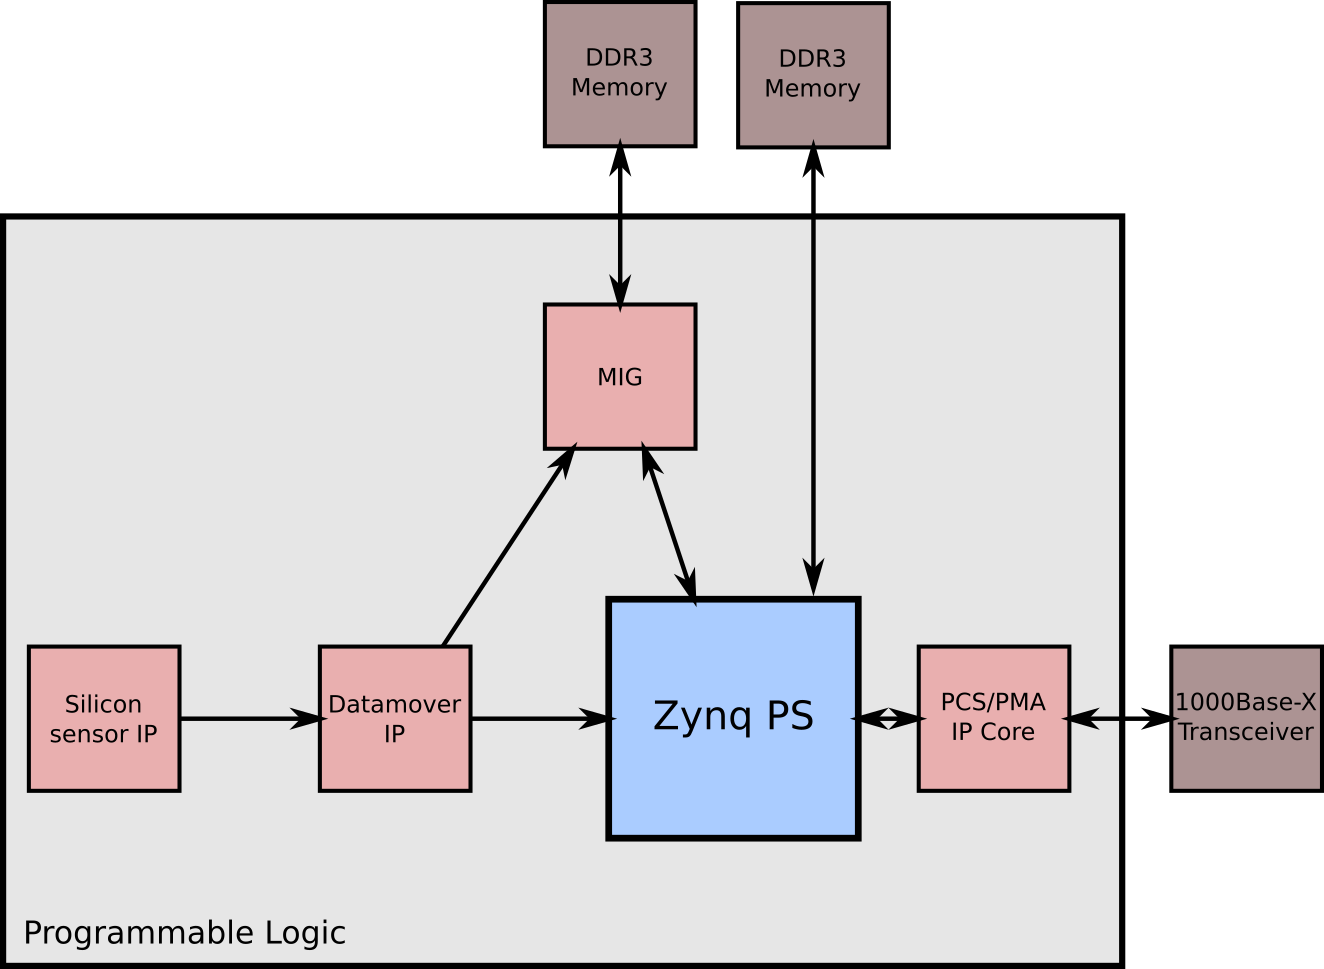
\includegraphics[width=5cm]{pic/silicon_arch.png}\\
            \caption{Counting arch.}
        \end{minipage}

    \end{frame}

    \begin{frame}{Realisation - CMV4000}
        \begin{figure}[H]
            \centering
            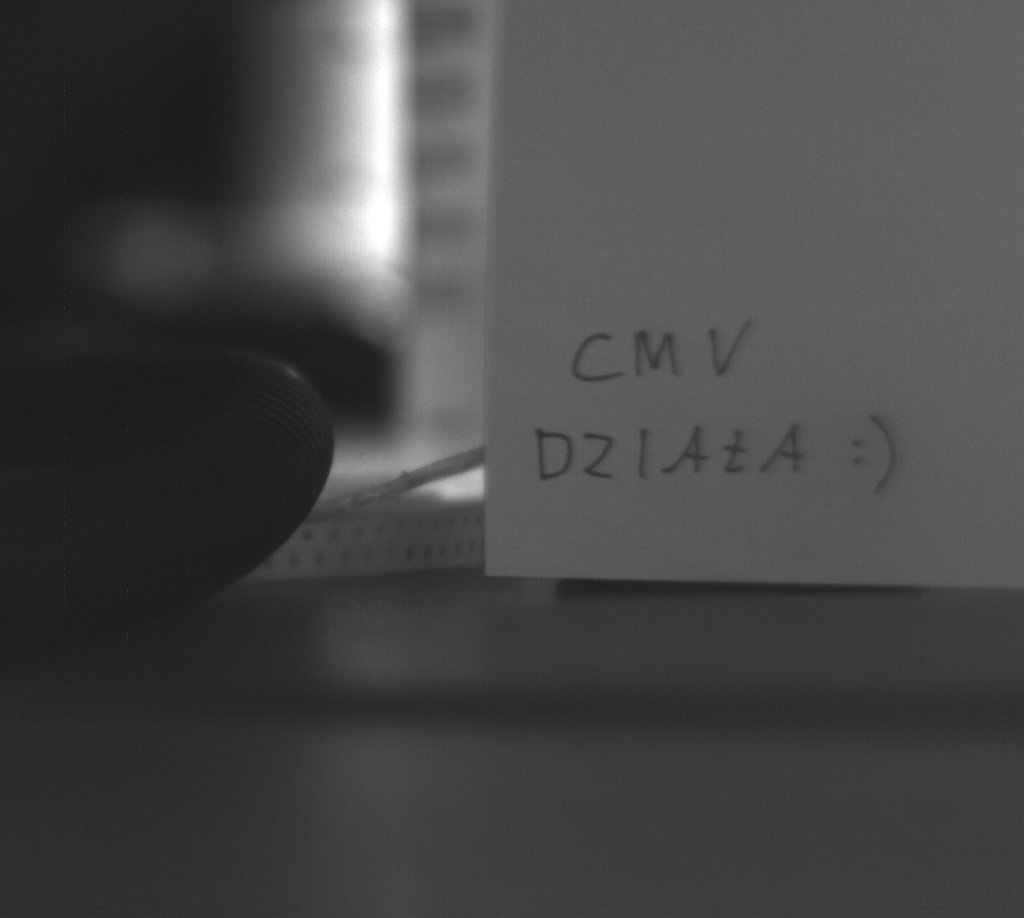
\includegraphics[width=10cm]{pic/test-0.jpg}
            \caption{Acquired image}
        \end{figure}
    \end{frame}

    \begin{frame}{Realisation - Counting sensor}
        \begin{figure}[H]
            \centering
            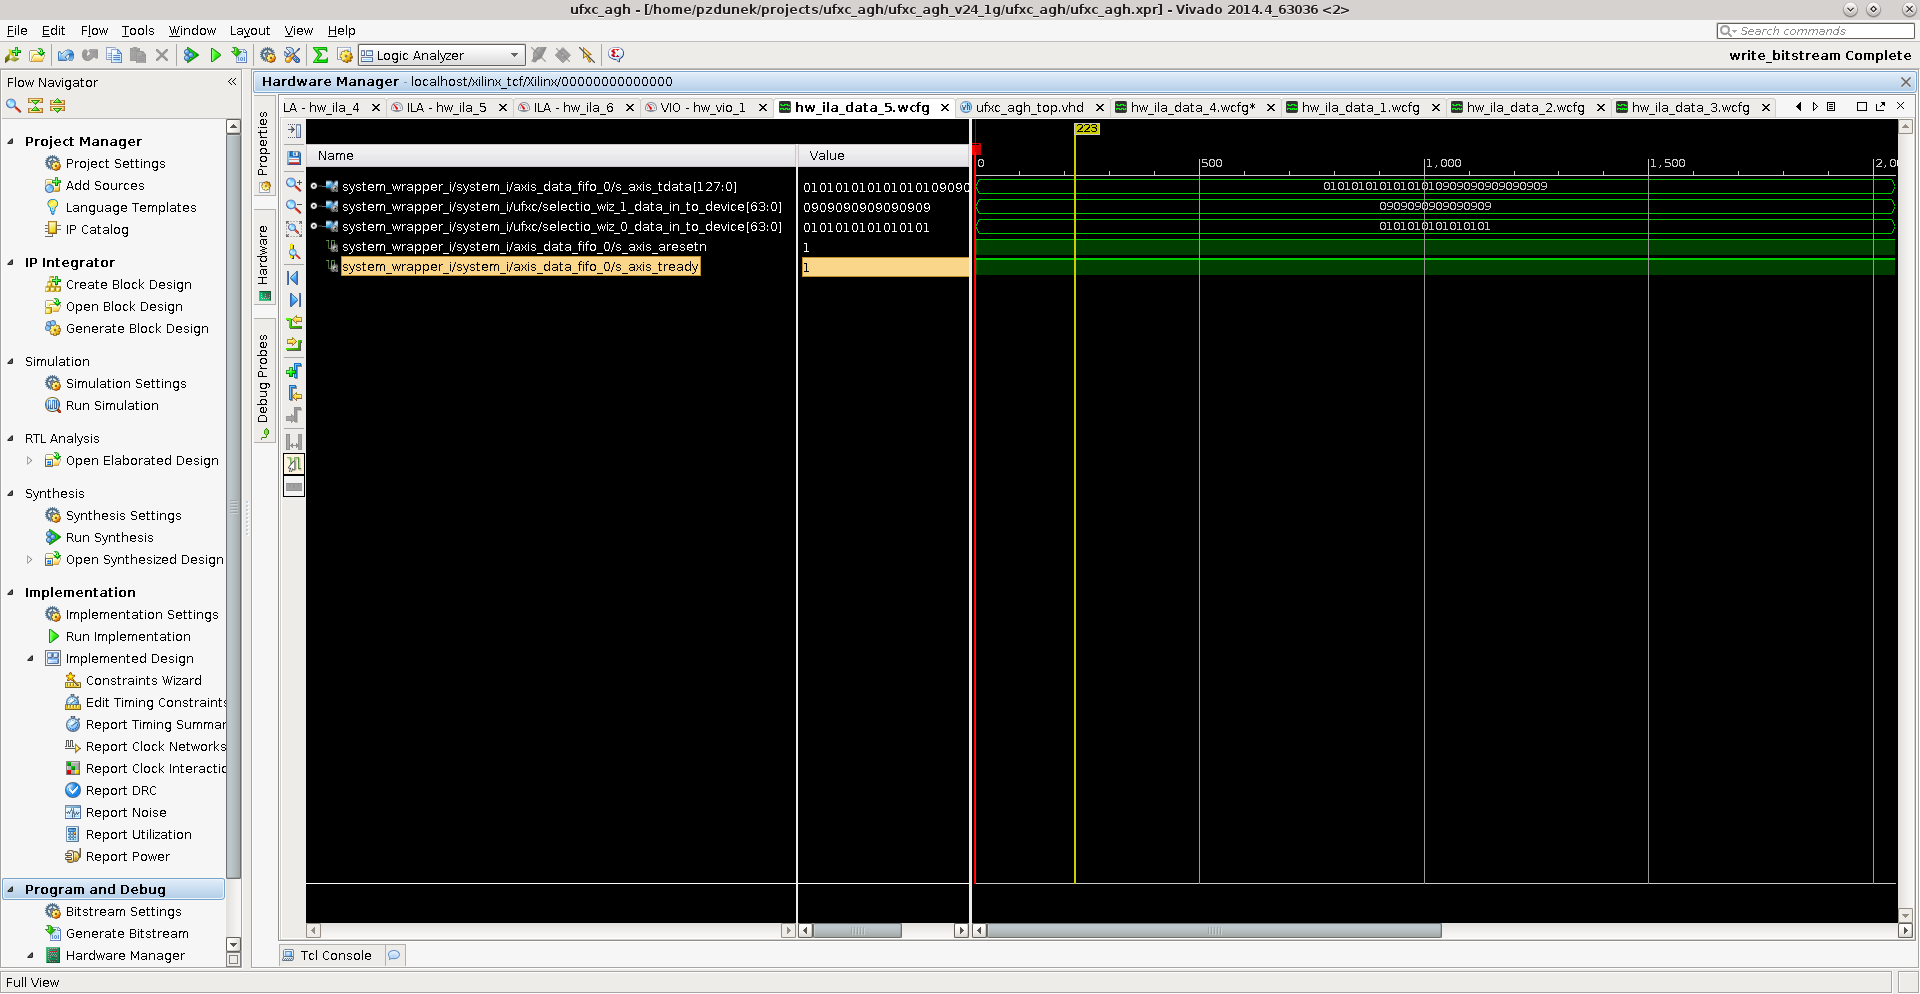
\includegraphics[width=10cm]{pic/out_get_fd.png}
            \caption{Readout from the sensor in the loopback mode}
        \end{figure}
    \end{frame}

    \begin{frame}{Summary}

        \begin{itemize}

            \item \textbf{Created framework can speed up development of scientific camera systems}

            \item \textbf{Modern SoC are a viable solution for embedded camera systems}

            \item \textbf{The FPGA fabric allows for using different types of sensors with the same hardware}

        \end{itemize}
        \vspace{1cm}
        Possible future upgrades:
        \begin{itemize}

            \item  10 Gbps Ethernet 
            \item  MLVDS bus synchronisation for IP Cores controlling the sensor - short range
            \item  White Rabbit synchronisation - for subnanosecond (up to 10 km) synchronisation 
        \end{itemize}

    \end{frame}


    \begin{frame}{Summary}
        \centering
        \LARGE{Thank you for your attention!}

    \end{frame}




    %  \begin{frame}{Typical camera overview}
    %      \begin{minipage}[t]{0.48\linewidth}
    %          Typical camera mainly consists of:
    %          \begin{itemize}
    %              \item optics
    %              \item shutter
    %              \item electronics
    %              \item shutter release
    %              \item sensor
    %              \item display
    %          \end{itemize}
    %      \end{minipage}\hfill
    %      \begin{minipage}[t]{0.48\linewidth}
    %          \begin{figure}[H]
    %              \centering
    %              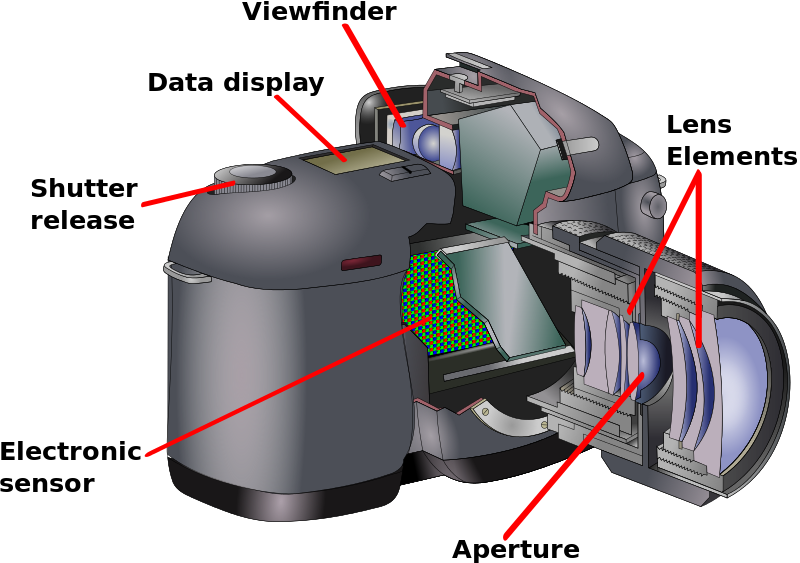
\includegraphics[width=5cm]{pic/camera.png}
    %              \caption{Example of camera system}
    %          \end{figure}
    %      \end{minipage}
    %  
    %  \end{frame}
    %  
    %  \begin{frame}{Scientific camera overview}
    %      \begin{minipage}[t]{0.48\linewidth}
    %          Scientific camera adds:
    %          \begin{itemize}
    %              \item multichannel operation
    %              \item high speed interface
    %              \item sophisticated sensor
    %              \item remote control
    %              \item no display :(
    %          \end{itemize}
    %      \end{minipage}\hfill
    %      \begin{minipage}[t]{0.48\linewidth}
    %          \begin{figure}[H]
    %              \centering
    %              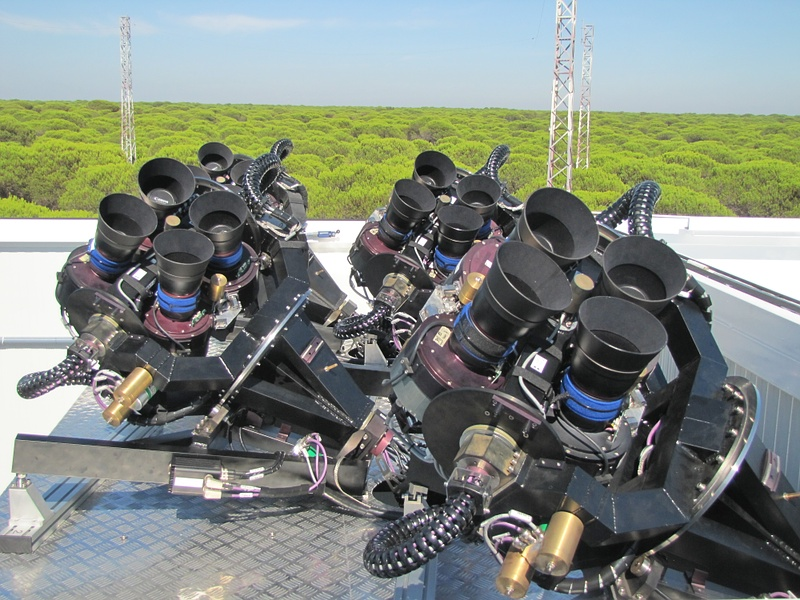
\includegraphics[width=5cm]{pic/camera_pi.jpg}
    %              \caption{Pi of the sky camera system}
    %          \end{figure}
    %      \end{minipage}
    %  
    %      \end{frame}

    %  \begin{frame}{Genesis}
    %      \begin{itemize}
    %          \item there is no open framework for camera design
    %          \item all designs are custom
    %          \item long and tedious development
    %          \item solution?
    %      \end{itemize}
    %  
    %  \end{frame}
    %  
    %  \begin{frame}{Goal of the master thesis}
    %      The goal of my thesis is to design a firmware for a scientific camera with the following                 requirements:
    %      \begin{itemize}
    %          \item high processing performance - for support of high resolutions
    %          \item ease of adding a support for a different sensor
    %          \item high speed communication - to send high amounts of data live
    %          \item multichannel operation - astronomical as well as medical applications require it
    %      \end{itemize}
    %  \end{frame}

    %\section{Concept of realization}
    %  \begin{frame}{Concept of realization}

    %          \begin{figure}[H]
    %              \centering
    %              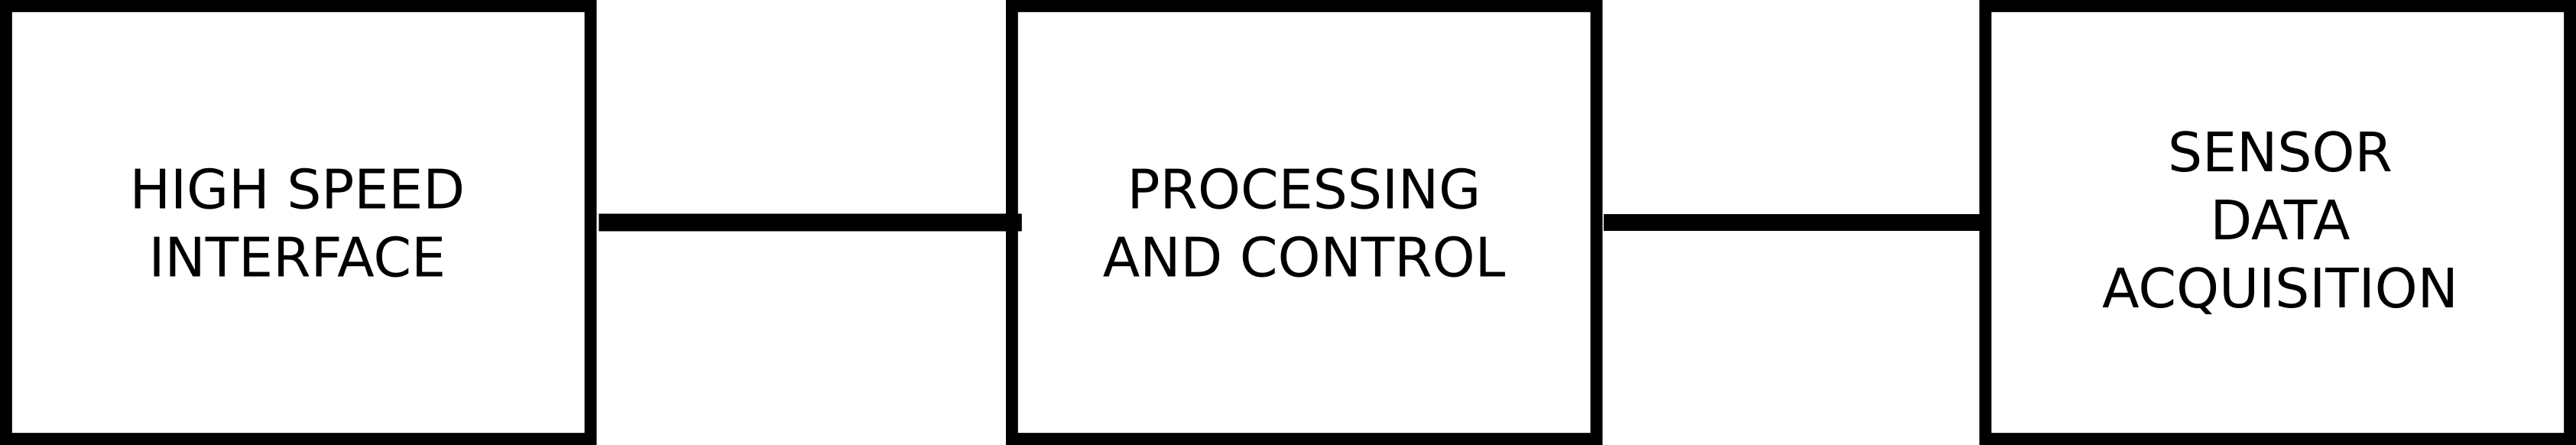
\includegraphics[width=10cm]{pic/camera_system_overview.png}
    %              \caption{High speed multichannel camera block diagram}
    %          \end{figure}

    %   \end{frame}
    %   
    %   \begin{frame}{Concept of realization}

    %          \begin{figure}[H]
    %              \centering
    %              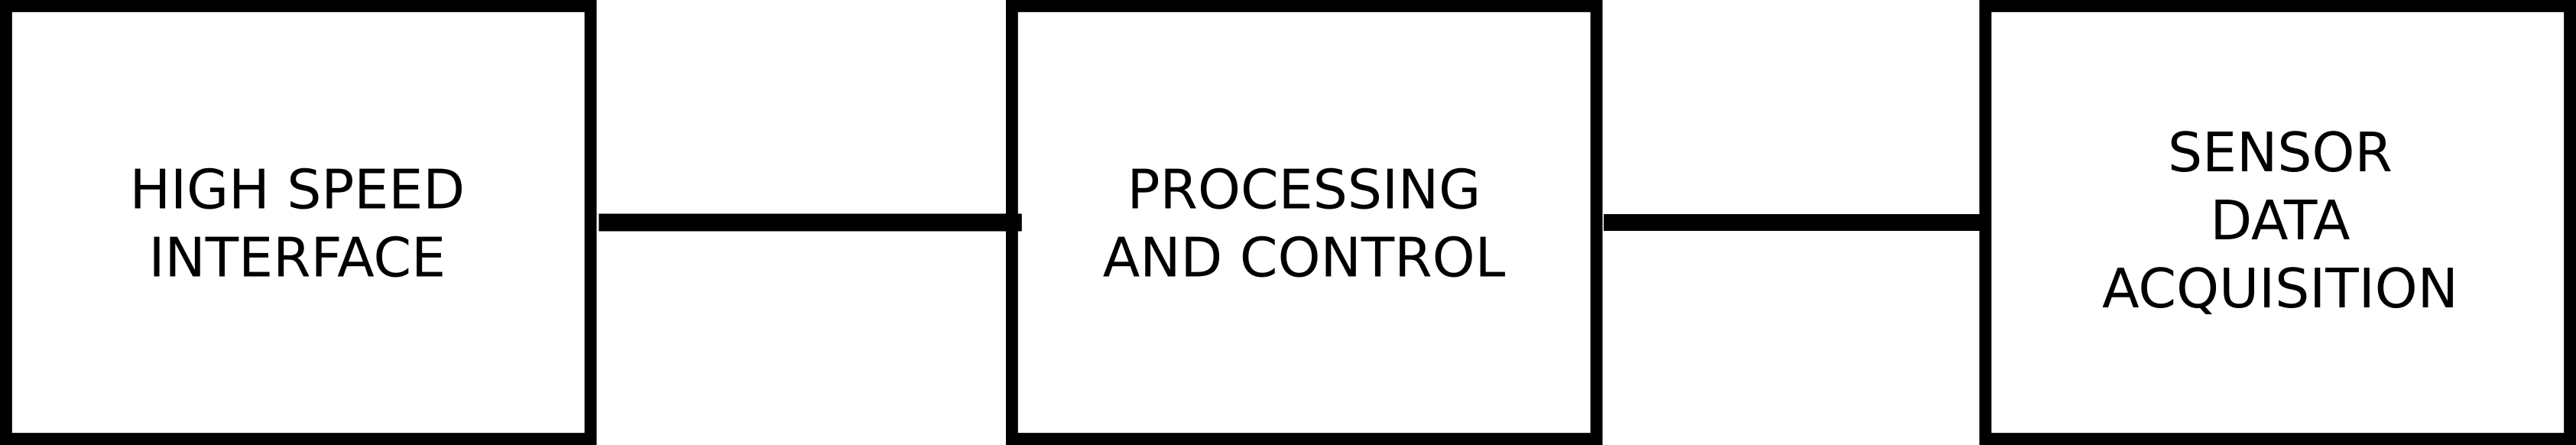
\includegraphics[width=10cm]{pic/camera_system_overview.png}
    %              \caption{High speed multichannel camera block diagram}
    %          \end{figure}
    %   \end{frame}
    %   

    %\section{Realization}
    %  \begin{frame}{dummy}

    %  \end{frame}
    %  

    %\section{Tests}
    %  \begin{frame}{dummy}

    %  \end{frame}
    %  

    \end{document}
